In this chapter the results for simple observable expectation values computed on the lattice gauge field ensembles that have been generated for this work, \cref{runs:ensembles}, are presented. Throughout the chapter, all error estimates associated to expectation values of observables have been computed using the bootstrap method, see \cref{app:resampling}, which is a popular resampling method used when the sample size of a statistical population is small, as is our case. The autocorrelation of data from the ensembles, introduced by the use of Markov chain to generate it, is handled using the procedure found in \cref{app:autocorr} as a correction to estimate of the variance proportional to the integrated autocorrelation time.

\section{Plaquette and Energy Density} 
The plaquette, \cref{plaquette}, and the energy density, \cref{eq:energy}, are tightly related as they both are estimates of the action of the gauge field.
%  We have already seen in \cref{sec:thermalization} that the plaquette can be used to check whether the metropolis algorithm has thermalized in the early stages of the chain. One could also study the dependence of the plaquette expectation value on the inverse coupling $\beta$ of the gluonic action. In \cref{fig:betplaq} the average plaquette computed for different inverse couplings. 
% \fig[0.7]{results/BetaPlaq.pdf}{Average Plaquette value as a bunction of the inverse coupling $\beta$.}{fig:betplaq}
Since the system is expected, after thermalization, to be at equilibrium, the sampling of the plaquette and of the energy density should be rather constant in Monte Carlo time. Figure \ref{fig:MCPlaqEnerg} shows that this is indeed the case.
\begin{figure}[hbt!]
    \centering
    \begin{subfigure}{0.45\textwidth}
        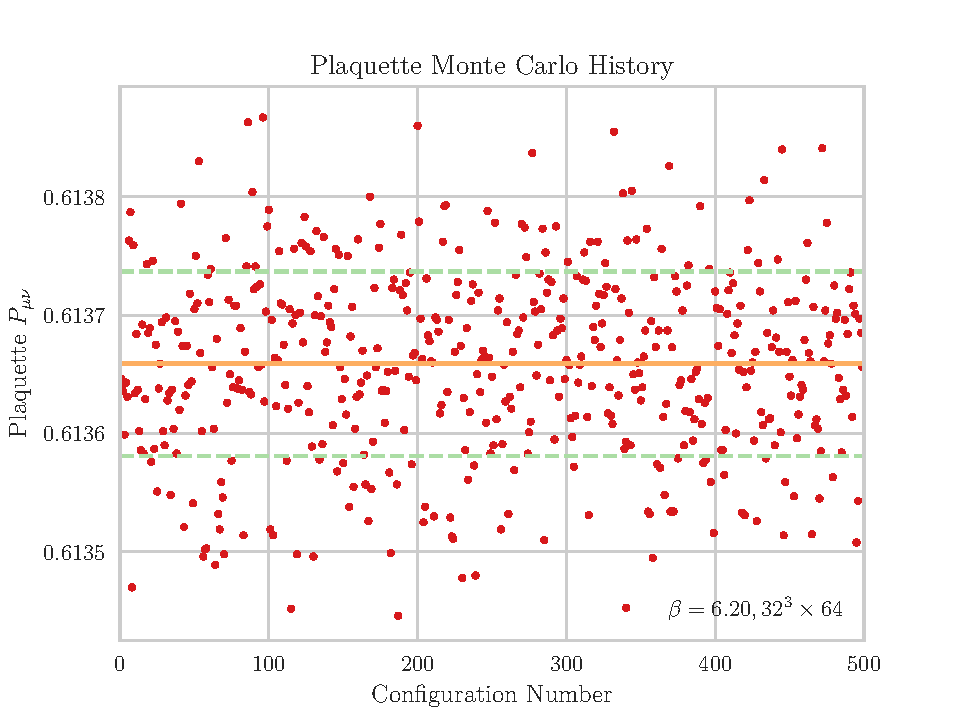
\includegraphics[width=\textwidth]{results/MCPlaq.pdf}
    \end{subfigure}
    \begin{subfigure}{0.45\textwidth}
        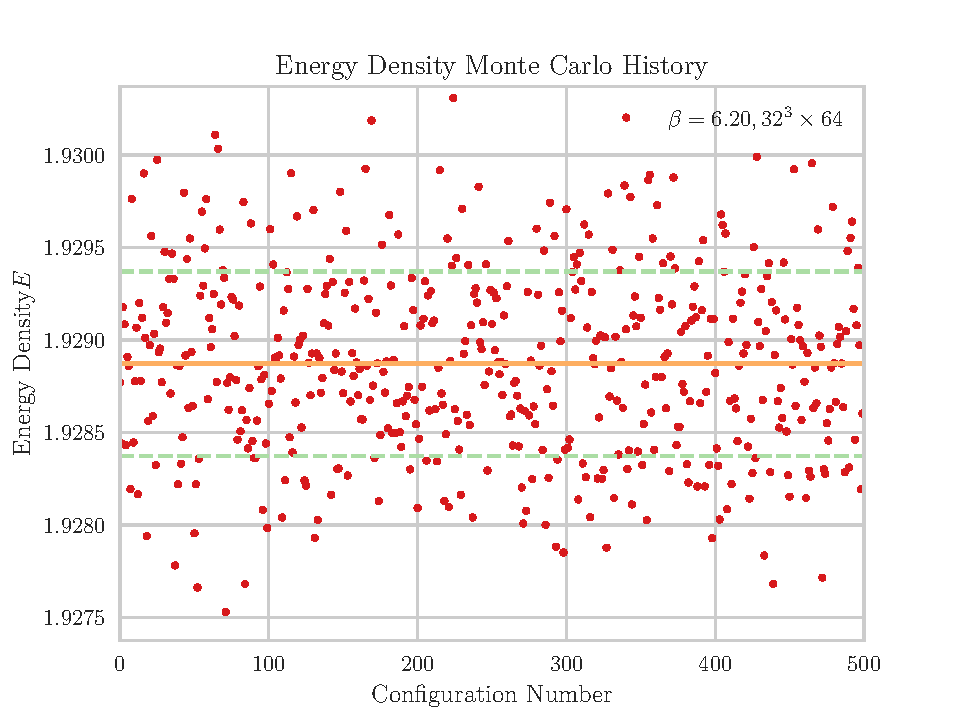
\includegraphics[width=\textwidth]{results/MCEnrg.pdf}
    \end{subfigure}
    \caption{\footnotesize Values for the Plaquette (left) and Energy Density (right) as a function of Monte Carlo time. The blue line is the average and the green dashed lines are the one $\sigma$ interval around it. The points represent the values of the two observables computed on every configuration of the ensemble. The average is thus the expectation value.}
    \label{fig:MCPlaqEnerg}
\end{figure}   

When applying the gradient flow equation:
\beq
\partial_{t_f} V_{t_f}(x,\mu) = - g_0^2 [\partial_{x,\mu}S_G(V_{t_f})]V_{t_f}(x,\mu),
\eeq
the configuration is evolved towards the minimum of the action. That implies that the values for the plaquette and the energy density at sufficiently large flow times are both lattice spacing and flow time independent. The results plotted in \cref{fig:plaq_plot} for the plaquette expectation value as a function of flow time, show that the gradient flow is indeed driving the gauge fields towards the stationary points. From the expression of the Wilson gluonic action, \cref{wilsonaction}, it is clear that the minimum of the action is reached when all the plaquettes are equal to the identity matrix. 
The expectation value of the average plaquette is therefore expected to be exactly one. 
\fig[0.7]{results/Plaquette.pdf}{Plaquette expectation value $\langle P_{\mu\nu} \rangle$ as a function of flow time $t_f$, here expressed in the form of the smearing radius $\sqrt{8t_f}$. The data for all the four ensembles of \cref{runs:ensembles} is shown. Errorbars are too small to be visible on the plot.}{fig:plaq_plot}

The energy density has an even simpler proportional relation to the action and \cref{fig:energy_plot} proves that the action is indeed minimized in the large flow time limit.

\fig[0.7]{results/Energy.pdf}{Energy density expectation value $\langle E\rangle$ as a function of gradient flow smearing radius $\sqrt{8t_f}$. The different data series represent the four different ensembles that have been generated, see \cref{runs:ensembles}. The errorbars not visible on the plot as they are small.}{fig:energy_plot}

As discussed in \cref{sec:obs_autocorr}, the integrated autocorrelation time of the observables is a crucial quantity to assess the quality of the results. We therefore computed $\tau_{int}$ for for the energies for all the different ensembles. We then looked at its flow time dependence. From \cref{fig:energyautocorr} we conclude that for all ensembles we generated the value of $\tau_{int}$ for the energy density never exceeds the value of one. This result is suggesting that the data we sampled for this observable is almost uncorrelated. Nevertheless, all results of this work (including \cref{fig:plaq_plot} and \cref{fig:energy_plot}) have variances corrected by $\tilde\sigma^2 = 2\tau_{int}\sigma^2$. The discontinuities in the integrated autocorrelation time stem from different truncations in the windowing procedure described in \cref{app:autocorr}. One can however notice that the values between the jumps are still compatible within the error estimate of $\tau_{int}$ given by \cref{eq:tauint_error}. 

\fig[0.7]{results/EnergyTauInt.pdf}{Integrated autocorrelation time of the Energy Density as a function of the smearing radius $\sqrt{8t_f}$. The discontinuity of the data is given by the approximation given by the truncation procedure described in \cref{app:autocorr}}{fig:energyautocorr} 

\section{Topological Charge}
Another interesting quantity to compute on our gauge fields is the topological charge, as defined in \cref{eq:topc}. In the continuum theory it assumes only integer values, with a distribution around zero that resembles a gaussian, though there are studies that prove that indeed it is not a normal distribution \cite{ce_non-gaussianities_2015}. \\
The topological charge on the lattice is affected by short range fluctuations given by discretization effects. The smoothing properties of the gradient flow on this observable removes the fluctuations and reveals the ``true'' value of the charge. An illustrative example is to plot the topological charge of one gauge field configuration as a function of the smearing radius. In \cref{fig:topcsingle} we show the evolution of the topological charge for three different gauge field configurations of lattice spacing $a=0.049$ fm ($\beta=6.45$). 
\fig[0.7]{results/TopcSingle.pdf}{Topological charge for three single gauge field configurations, taken at random from the $\beta=6.45$ ensemble, plotted against the smearing radius $\sqrt{8t_f}$ of the gradient flow.}{fig:topcsingle}

We can notice that for all the three considered configurations the topological charge has a plateau at a smearing of roughly $0.15$ fm. The value, for this example, corresponds to approximately three times the lattice spacing.\\ 
For some configurations however, especially for larger lattice spacings, the plateau is not clear and defined. The explanation could be the too simple definition that has been used for the gauge field strength tensor. Perhaps an improved definition of the tensor, given for example by a linear combination of plaquettes and larger Wilson Loops could be beneficial\cite{alexandrou_comparison_2017}. These higher order definitions of $G_{\mu\nu}(n)$ can be systematically constructed to cancel the $\mathcal{O}(a^2)$ errors that we have in the current definition. A simple example is to include Wilson loops of size $1\times1$ (the plaquettes),  $2\times1$ and $1\times2$ (minimal rectangles). The topological charge density would then become:
\beq
    q^{imp}(n) = \frac{1}{32\pi^2} c_0 \epsilon^{\mu\nu\rho\sigma}\Tr [G_{\mu\nu}^{(clover)}(n)G_{\rho\sigma}^{(clover)}(n)] + c_1 \epsilon^{\mu\nu\rho\sigma}\Tr [G_{\mu\nu}^{(rect)}(n)G_{\rho\sigma}^{(rect)}(n)],
\eeq
where $G_{\mu\nu}^{(rect)}(n)$ represents the sum of all Wilson loops in the plane $\mu\nu$ of side 2. The coefficients $c_0$ and $c_1$ are set by looking at the expansion of $G_{\mu\nu}^2(x)$ on the lattice. This potential improvement could be a future addition to our program.

When considering the expectation value of the topological charge of an ensemble, we expect its value to be zero \cite{ce_non-gaussianities_2015}. From \cref{fig:topc} one can check that our data for the expectation value of $\langle Q\rangle$ is in fact within error-bars always compatible with zero. 
\fig[0.7]{results/TopChar.pdf}{Topological charge expectaion value $\langle Q\rangle$ as a function of the smearing radius $\sqrt{8t_f}$. Errorbars are computed using bootstrap and corrected with the integrated autocorrelation time correction factor.}{fig:topc}

We should note that the increasing error-bars, for $\beta = 6.2$ and $\beta = 6.45$ in particular, are given by the decreasing, with respect to the $\beta=6.00$ and $\beta=6.10$ cases, ensemble size and the increasing integrated autocorrelation time $\tau_{int}$. The latter, in particular, is used as a correction to the estimate of the variance. \\
In \cref{fig:topctauint} we plot the integrated autocorrelation time of the topological charge as a function of flow time. If compared to the analog plot the energy density (\cref{fig:energyautocorr}) one can notice tht the two observables have very different autocorrelation times. The topological charge not only has a much larger $\tau_{int}$ on the lattice, but it grows rapidly with the inverse lattice spacing. It should be noted that the value of $N_{corr}$, the Monte Carlo updates between two data points, is much larger for the $\beta=6.45$ ensemble than all the others, but nevertheless the $\tau_{int}$ is by far larger.
\fig[0.7]{results/TopcTauInt.pdf}{Integrated autocorrelation time $\tau_{int}$ of the topological charge as a function of the gradient flow smearing radius $\sqrt{8t_f}$. The ensembles are the ones reported in \cref{runs:ensembles}.}{fig:topctauint}

One last consideration on the topological charge is the comparison of its distribution at zero flow time and the one in the large flow time limit. In \cref{fig:topchist} we show two histograms of such distributions for the $\beta = 6.20$ ensemble at $\sqrt{8t_f} = 0$ fm and $\sqrt{8t_f} = 0.6$ fm respectively. The bins are taken to be centered on integer and half-integer values in order to capture differences of the distribution of the topological charge. In the continuum, only integer values should be allowed, while on the lattice, due to discretization, the topological charge is in general not an integer. However, from \cref{fig:topchist} it is possible to see that the gradient flow estimate of the charge has a distribution with much sharper peaks around integer values, rather than half-integer ones, if compared to the zero flow time distribution. 
\begin{figure}[hbt!]
    \centering
    \begin{subfigure}{0.7\textwidth}
        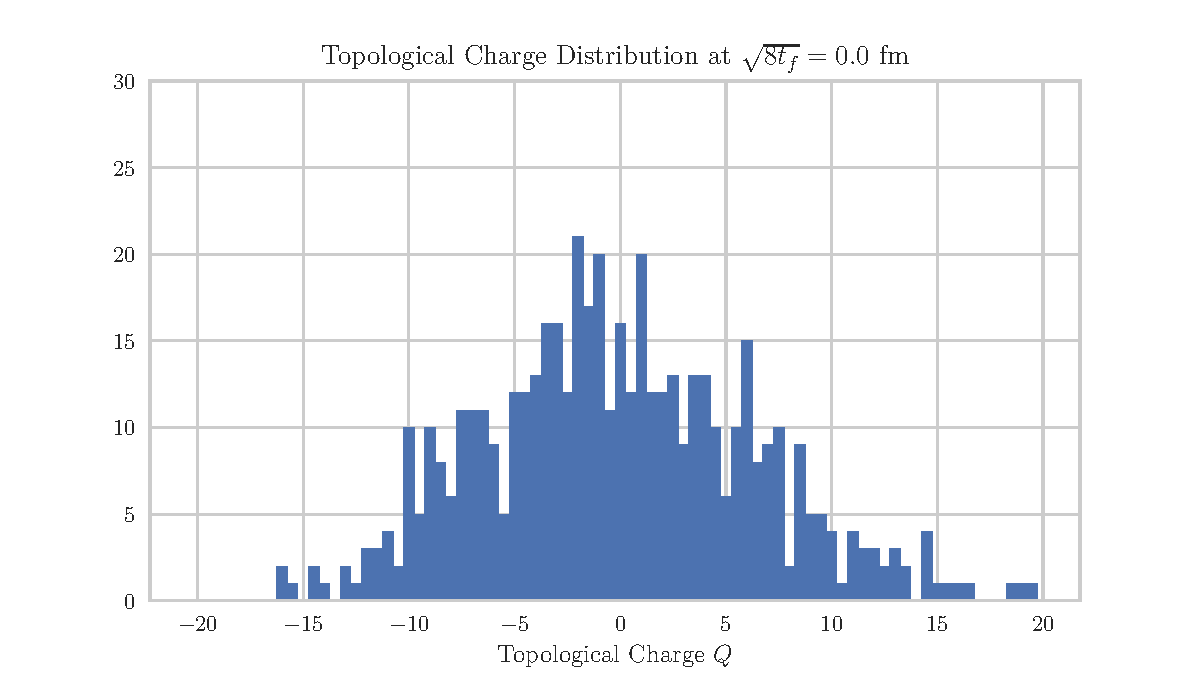
\includegraphics[width=\textwidth]{results/TopcHistNoFlow.pdf}
    \end{subfigure}
    \begin{subfigure}{0.7\textwidth}
        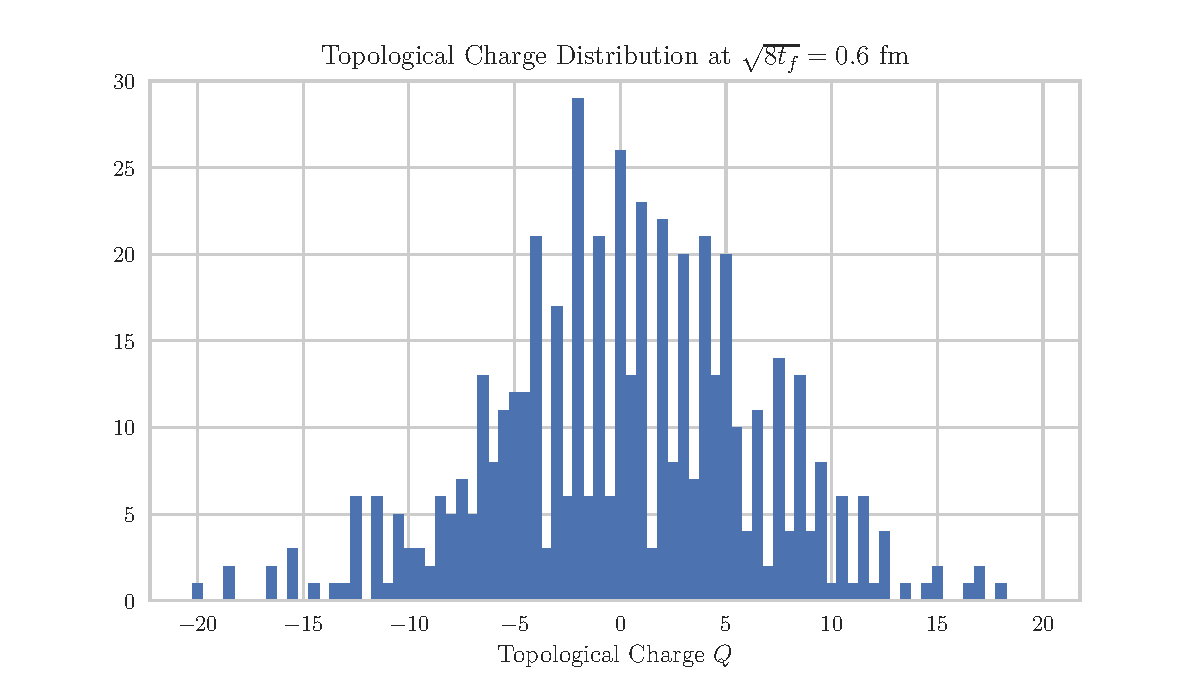
\includegraphics[width=\textwidth]{results/TopcHistFlow.pdf}
    \end{subfigure}
    \caption{\footnotesize Histograms of the topological charge values at $\sqrt{8t_f} = 0$ fm (top) and $\sqrt{8t_f} = 0.6$ fm (bottom) for the $\beta=6.20$ ensemble. The bins are centered on integers and half-integer values.}
    \label{fig:topchist}
\end{figure} 

\section{Topological Susceptibility}
The last physical quantity that we present in this chapter is the topological susceptibility, \cref{eq:tops}. Being proportional to the expectation value of the squared topological charge, it is related to the width of the distributions in \cref{fig:topchist}. The evolution with the gradient flow of the susceptibility is not trivial. At low flow times the high-frequency fluctuations in the topological charge make the expectation value of the susceptibility diverge. The smoothing property of the gradient flow remove the fluctuations revealing the real value of the quantity. In \cref{fig:tops} the flow time evolution of the topological susceptibility is shown.
\fig[0.7]{results/TopSusc.pdf}{Topological susceptibility $\chi^{1/4}$ as a function of the smearing radius $\sqrt{8t_f}$, for all the ensembles generated for this work.}{fig:tops} 
 
The value of $\chi^{\frac{1}{4}}$, as defined in \cref{eq:topsus} has the physical units of energy, hence it is reported in MeV. We notice that for all ensembles in the large flow time limit the topological charge has a well defined plateau. It is then possible to take the continuum limit in a region between $0.4$ fm and $0.6$ fm. \\
The behavior at zero flow time is not what we were expecting, comparing for example to ref. \cite{shindler_nucleon_2015} we don't observe a clear divergency at $\sqrt{8t_f} = 0$ fm. The behavior seems to be more and more divergent (a true divergency is impossible, it is always a finite quantity on the lattice) for larger values of $\beta$. A possible explanation of this behavior is the usage of the clover definition of the gauge field strength tensor. Being the topological charge, at zero flow time, dominated by high-frequency fluctuations, the use of only $1\times1$ Wilson loops (the four plaquettes of the clover, \cref{fig:clover}) in the definition of $G_{\mu\nu}$ could be a problem. In the reference the field strength tensor was computed including loops up to size three, this could be the cause of difference in the low-flow time behavior. This low flow time dependence of the susceptibility on the definition of the field strength tensor should be investigated more. \\
From \cref{fig:tops} one can infer that the continuum limit, to recover the physical value of the topological susceptibility, can be taken by considering the value of the observable over an interval of the smearing radius between  $\sqrt{8t_f} = 0.4$ and $0.6$ fm. The extrapolation to the continuum has to be performed by using the dimensionless quantity $(a/r_0)^2$, with $a$ being the lattice spacing and $r_0 = 0.5$ fm the Sommer parameter \cite{guagnelli_precision_1998}. The ratio is taken squared in order to match the lattice units of the quantity that is being extrapolated, the susceptibility in this case (which is proportional to an energy). In \cref{fig:topscontlimit} the continuum limit of the topological susceptibility is taken using the values found for $\sqrt{8t_f}=0.5$ fm.   

\fig[0.7]{results/TopsContLimit.pdf}{Continuum limit extrapolation of $\chi^{\frac{1}{4}}$ from the values at $\sqrt{8t_f}=0.5$ fm. The fit is performed using the dimensionless quantity $(a/r_0)^2$ as a reference. The black point is the extrapolated point.}{fig:topscontlimit}

The value we obtain for the extrapolated topological susceptibility is:
\beq
    \chi^{\frac{1}{4}} = 186.9(4.9)~\text{MeV} .
    \label{val:tops}
\eeq 
This is compatible with the value in \cite{shindler_nucleon_2015} of  $\chi^{\frac{1}{4}} = 195.9(4.9)~\text{MeV} $. \NOTE{PROBLEMS; B=6.0 POINT; MATHIAS}

As an additional result we can use this extrapolation to compute the mass of the $\eta'$ meson taken from the Witten-Veneziano formula \cite{witten_current_1979}:
\beq
    \chi = \frac{F_\pi^2m_{\eta'}^2}{2N_{flavors}}.
\eeq 
Using as inputs $F_\pi = 92$ MeV, the pion decay constant, and having $N_{flavors} = 3$, we find the mass of the $\eta'$ meson to be:
\beq    
    m^{(lattice)}_{\eta'} = \sqrt{\frac{\chi^{\frac{1}{4}} 2N_{flavors}}{F_\pi^2}} = 921(16)~\text{MeV},
\eeq
which we compare with an experimental value  $m^{(exp)}_{\eta'} = 957.78(6)$ MeV, so we are off by more than $2\sigma$, but probably the result is largely influenced by the data point obtained from $\beta=6.45$, which has less statistics (only 250 configurations) and larger uncertainty.